% ============================================================
%  SCIENTIFIC REPORT TEMPLATE
%  Compile with: pdflatex -> bibtex -> pdflatex -> pdflatex
% ============================================================

\documentclass[12pt, a4paper]{article}

% ── Encoding & Fonts ─────────────────────────────────────────
\usepackage[T1]{fontenc}
\usepackage[utf8]{inputenc}
\usepackage{lmodern}
\usepackage{microtype}          % Better typography

% ── Page Layout ──────────────────────────────────────────────
\usepackage[
  top=25mm, bottom=25mm,
  left=25mm, right=25mm,
  headheight=14pt
]{geometry}

% ── Headers & Footers ────────────────────────────────────────
\usepackage{fancyhdr}
\pagestyle{fancy}
\fancyhf{}

\cfoot{\thepage}
\renewcommand{\headrulewidth}{0.4pt}

% ── Mathematics ──────────────────────────────────────────────
\usepackage{amsmath, amssymb, amsthm}
\usepackage{mathtools}

% ── Figures & Tables ─────────────────────────────────────────
\usepackage{graphicx}
\usepackage{float}
\usepackage{booktabs}           % Professional table rules
\usepackage{tabularx}
\usepackage{multirow}
\usepackage{caption}
\usepackage{subcaption}
\captionsetup{font=small, labelfont=bf, skip=6pt}

% ── Colours ──────────────────────────────────────────────────
\usepackage[dvipsnames]{xcolor}
\definecolor{linkblue}{RGB}{0, 74, 153}

% ── Hyperlinks ───────────────────────────────────────────────
\usepackage[
  colorlinks=true,
  linkcolor=linkblue,
  citecolor=linkblue,
  urlcolor=linkblue,
  pdftitle={Scientific Report Title},
  pdfauthor={Author Names}
]{hyperref}

% ── References ───────────────────────────────────────────────
\usepackage[numbers, sort&compress]{natbib}
\bibliographystyle{unsrtnat}

% ── Code Listings ────────────────────────────────────────────
\usepackage{listings}
\lstset{
  basicstyle=\ttfamily\small,
  breaklines=true,
  frame=single,
  backgroundcolor=\color{gray!8},
  commentstyle=\color{OliveGreen},
  keywordstyle=\color{Blue}\bfseries,
  stringstyle=\color{BrickRed},
  numbers=left, numberstyle=\tiny\color{gray},
  numbersep=6pt
}

% ── Misc Packages ────────────────────────────────────────────
\usepackage{enumitem}
\usepackage{lipsum}             % Placeholder text — remove in final draft
\usepackage{siunitx}            % SI units: \SI{9.8}{\metre\per\second\squared}
\usepackage{chemformula}        % Chemical formulas: \ch{H2O}
\usepackage{lineno}             % Line numbers (comment out for final)
% \linenumbers

% ── Theorem Environments ─────────────────────────────────────
\theoremstyle{plain}
\newtheorem{theorem}{Theorem}[section]
\newtheorem{lemma}[theorem]{Lemma}
\theoremstyle{definition}
\newtheorem{definition}{Definition}[section]
\theoremstyle{remark}
\newtheorem{remark}{Remark}

% ── Custom Commands ──────────────────────────────────────────
\newcommand{\eg}{\textit{e.g.},\ }
\newcommand{\ie}{\textit{i.e.},\ }
\newcommand{\etal}{\textit{et al.}}
\newcommand{\vect}[1]{\boldsymbol{#1}}
\newcommand{\diff}{\mathrm{d}}   % upright d for integrals

% ============================================================
%  TITLE PAGE METADATA
% ============================================================
\title{
  \vspace{-1.5cm}
  {\Large \textbf{Gravitational Lense-Thirring Effect}} \\[6pt]
  {\large Lense-Thirring Analogous to Electromagnetism}
}


% ============================================================
\begin{document}
% ============================================================

\maketitle
\thispagestyle{empty}

% ── Abstract ─────────────────────────────────────────────────
\begin{abstract}
  \noindent
  Rotating masses in general relativity produce subtle effects on the surrounding spacetime that are not predicted by classical Newtonian gravity. One such phenomenon is the Lense–Thirring effect, in which the rotation of a massive body leads to the dragging of spacetime, producing measurable deviations in the motion of nearby objects. This report examines the theoretical basis of the Lense–Thirring effect and its mathematical formulation within the framework of general relativity. Under the weak-field approximation, the Einstein field equations can be expressed in a form analogous to Maxwell’s equations of electromagnetism. By analyzing the resulting equations and solving the geodesic equation in this regime, the gravitational field can be separated into scalar and vector components that resemble electric and magnetic fields in electromagnetism. The scalar component corresponds to the classical Newtonian gravitational potential, while the vector component represents a gravitomagnetic field arising from the rotation of the mass. Although this gravitomagnetic contribution is extremely weak and difficult to detect, precise experimental measurements have confirmed its existence. The study highlights the analogy between gravitation and electromagnetism in the weak-field limit and illustrates how frame-dragging effects provide important observational support for the predictions of general relativity.
  



  \vspace{6pt}
  
\end{abstract}

\noindent\rule{\linewidth}{0.4pt}
\tableofcontents
\noindent\rule{\linewidth}{0.4pt}

\newpage

% ============================================================
\section{Introduction}
\label{sec:introduction}
Newton formulated the law of universal gravitation in the late seventeenth century, providing a successful description of gravitational interactions between massive bodies. However, the development of electromagnetic theory in the nineteenth century and experiments such as the Michelson–Morley experiment revealed inconsistencies within classical physics. In the early twentieth century, Albert Einstein introduced the special theory of relativity, which fundamentally changed the understanding of space and time. While special relativity successfully explained many phenomena at high velocities, it did not incorporate gravity, motivating the later development of the general theory of relativity.

While special relativity successfully explained many physical phenomena, it did not incorporate acceleration or gravity. The theory is formulated in flat spacetime and therefore cannot account for gravitational effects such as gravitational redshift or the motion of bodies under gravity. To address this limitation, Albert Einstein introduced the equivalence principle, which states that in sufficiently small regions of spacetime the laws of physics reduce to those of special relativity. This principle suggests that gravity can be understood as a geometric property of spacetime rather than a conventional force. The motion of freely falling particles in such a curved spacetime is described by the geodesic equation. 
\begin{equation}
  \frac{d^2x^{\alpha}}{d{\tau}^2}+{\Gamma}^{\alpha}_{\beta \gamma}\frac{dx^{\beta}}{d {\tau}}\frac{dx^{\gamma}}{d {\tau}}=0
  \label{eq: Geodesics Equation}
\end{equation}
To determine how spacetime itself is curved by the presence of mass and energy, Einstein formulated the Einstein field equations.
\begin{equation}
  {G^{\alpha \beta}}+{\Lambda}g^{\alpha \beta } =\frac{8{\pi}G{T^{\alpha \beta}}}{c^4}
  \label{eq: Einstein Field Equation}
\end{equation}

The Lense–Thirring effect is of particular interest because it has been experimentally measured using satellite missions such as LAGEOS, which detected the frame-dragging of spacetime caused by Earth’s rotation. Such observations provide important experimental confirmation of the predictions of general relativity.

This report examines the weak-field approximation of general relativity and its application to slowly rotating massive bodies, which leads to equations analogous to those of electromagnetism. The objective of this work is to analyze and illustrate the resulting gravitomagnetic effects associated with the Lense–Thirring phenomenon.

% ============================================================
\section{Derivation}
\label{sec:Derivation }
% ============================================================

\subsection{The Weak-Field Approximation}
\label{subsec:The Weak-Field Approximation}
Space-time is considered to be nearly flat. 
\begin{equation}
  g_{\mu \nu}=\eta_{\mu \nu}+h_{\mu \nu}
  \label{eq: Perturbation}
\end{equation}
We assume $ \|h_{\mu\nu}\| \ll 1 $ for the linearized approximation. It's called nearly Lorentz co-ordinates. This is similar to freely falling frame.
Since the space-time metric is a tensor.
\begin{equation}
    g_{{\bar{\mu}} {\bar{\nu}} }=\frac{\partial x^\alpha}{\partial x^{\overline{\mu}}}\frac{\partial x^\beta}{\partial x^{\overline{\nu}}}g_{\alpha \beta}
    \label{eq: Perturbation}
\end{equation}

\begin{equation}
    \Lambda^{\alpha}_{\bar\mu} =\frac{\partial x^{\alpha}}{\partial x^{\bar\mu}}
\end{equation}
The metric tensor could be assumed like a tensor field over a flat space-time where $h_{\mu \nu}$ is the field in the background. It is the same under transformation.
\begin{equation}
    g_{\bar\mu \bar\nu} =\eta_{\bar\mu \bar\nu}+ h_{\bar\mu \bar\nu}
\end{equation}
Gauge transformation in linearised gravity. We consider a tiny transformation $\xi<<1$ where we add a slight curve to flat space-time.
\begin{equation}
    {x'}^\alpha = x^\alpha+\xi^\alpha(x^\beta)
\end{equation}
\begin{equation}
    L^{\alpha'}_\beta = \delta^\alpha_\beta + {\partial_\beta\xi^\alpha}
\end{equation}
Since it's an infinitesimally small coordinate transformation, the inverse
\begin{equation}
    L^{\alpha}_{\beta'} =  \delta^\alpha_{\beta'} - {\partial_{\beta'}\xi^\alpha}+\mathcal{O}({\partial}\xi^2)
\end{equation}
The metric tensor transforms to.
\begin{equation}
    g_{\bar\mu \bar\nu}=L^\alpha_{\bar\mu}L^\beta_{\bar\nu}g_{\alpha \beta}
\end{equation}
It simplifies to 
\begin{equation}
    g_{\bar\mu \bar\nu}=\eta_{\mu \nu}+h_{\mu \nu}-{\partial_\mu \xi_\nu}-{\partial_\nu \xi_\mu}+\mathcal{O}({\partial \xi^2})
\end{equation}
The perturbation transforms to
\begin{equation}
    h_{\mu \nu}\xrightarrow{}h_{\mu \nu}-{\partial_\mu \xi_\nu}-{\partial_\nu \xi_\mu}
\end{equation}
The Riemann Tensor is given by
\begin{equation}
    R^\alpha_{\beta \gamma \delta}={\partial_\gamma \Gamma^{\alpha}_{\delta \beta}}-{\partial_\delta \Gamma^{\alpha}_{\gamma \beta}}+\Gamma^\alpha_{\gamma \epsilon}\Gamma^\epsilon_{\delta \beta}-\Gamma^\alpha_{\delta \epsilon}\Gamma^\epsilon_{\gamma \beta}
\end{equation}
Applying the gauge transformation results in
\begin{equation}
    R_{\alpha \beta \gamma \delta}=\frac{1}{2}({\partial_\beta}{\partial_\gamma}h_{\alpha \delta}+{\partial_\alpha}{\partial_\delta}h_{\beta \gamma}-{\partial_\beta}{\partial_\delta}h_{\alpha \gamma}-{\partial_\alpha}{\partial_\gamma}h_{\beta \gamma})
\end{equation}
It is found to be invariant under this gauge transformation. The Ricci tensor is given by
\begin{equation}
    R_{\alpha \beta}=\eta^{\mu \nu}R_{\mu \alpha \nu \beta}
\end{equation}
Under the gauge transformation
\begin{equation}
    R_{\alpha \beta}=\frac{1}{2}({\partial_\alpha}{\partial^\mu}h_{\mu \beta}+{\partial_\beta}{\partial^\mu}h_{\mu \alpha}+{\partial_\alpha}{\partial_\beta}h-\Box{h_{\alpha \beta}})
\end{equation}
The Ricci scalar is given by
\begin{equation}
    R=\eta^{\alpha \beta}R_{\alpha \beta}={\partial^\alpha}{\partial^\mu}h_{\mu \alpha}-\Box{h}
\end{equation}
The Linearized Einstein curvature tensor  
\begin{equation}
    G_{\alpha \beta}=R_{\alpha \beta}-\frac{1}{2}\eta_{\alpha \beta}R
\end{equation}
Turns in to
\begin{equation}
    G_{\alpha \beta}=\frac{1}{2}({\partial_\alpha}{\partial^\mu}h_{\mu \beta}+{\partial_\beta}{\partial^\mu}h_{\mu \alpha}+{\partial_\alpha}{\partial_\beta}h-\Box{h_{\alpha \beta}} -\eta_{\alpha \beta}{\partial^\alpha}{\partial^\mu}h_{\mu \alpha}+\eta_{\alpha \beta}\Box{h})
\end{equation}

And by making a substitution similar to the relation between Ricci tensor and Einstein curvature tensor
\begin{equation}
    \bar h_{\alpha \beta}=h_{\alpha \beta}-\frac{1}{2}\eta_{\alpha \beta}h
    \label{eq:red_per}
\end{equation}
Multiplying  $\eta^{\alpha \beta}$  in \eqref{eq:red_per}
\begin{equation}
    \bar{h} = \eta^{\mu\nu}\bar{h}_{\mu\nu} = h - \frac{1}{2}(4)h = h - 2h = -h
\end{equation}

So $\bar{h} = -h$, which means $h = -\bar{h}$. Substituting back:

\begin{equation}
    h_{\mu\nu} = \bar{h}_{\mu\nu} - \frac{1}{2}\eta_{\mu\nu}\bar{h}
    \label{eq:hii}
\end{equation}
\
The Linearized Einstein curvature tensor turn into
\begin{equation}
\begin{aligned}
G_{\alpha\beta} &= \frac{1}{2}(\partial_\alpha \partial_{\bar{\mu}} \bar{h}^{\mu}{}_{\beta} + \frac{1}{2}\eta_{\mu\beta}\partial_\alpha \partial^\mu h + \partial_\beta \partial_{\bar{\mu}} \bar{h}^{\mu}{}_{\alpha} + \frac{1}{2}\eta_{\mu\alpha}\partial_\beta \partial^\mu h \\
&\quad - \partial_\alpha \partial_\beta h - \Box \bar{h}_{\alpha\beta} - \frac{1}{2}\eta_{\alpha\beta}\Box h + \eta_{\alpha\beta}\Box h \\
&\quad - \eta_{\alpha\beta}\partial_\mu \partial_\nu \bar{h}^{\mu\nu} - \frac{1}{2}\eta_{\alpha\beta}\eta_{\mu\nu}\partial^\mu \partial^\nu h)
\end{aligned}
\end{equation}
It simplifies to 
\begin{equation}
G_{\alpha\beta} = \frac{1}{2}(\partial_\alpha\partial_{\bar{\mu}}\bar{h}^{\mu}{}_{\beta} + \partial_\beta\partial_{\bar{\mu}}\bar{h}^{\mu}{}_{\alpha} - \eta_{\alpha\beta}\partial_\mu\partial_\nu\bar{h}^{\mu\nu} - \Box\bar{h}_{\alpha\beta})
\end{equation}
To make the equation in a better form, use the freedom gauge transformation.  
\begin{equation}
    \partial^\mu \bar h_{\mu \nu}=0
\end{equation}
The field equation turns into
\begin{equation}
    \Box{\bar h_{\alpha \beta}}=-16\pi GT_{\alpha \beta}
\end{equation}
\subsection{Lense-Thirring Effect}
When considering slowly rotating massive bodies such as Earth, the gravitational field is relatively weak and the resulting spacetime curvature is small. In such situations it is appropriate to apply the weak-field approximation to the Einstein field equations. The smallness of the curvature can be understood from the factor $\frac{G\pi}{c^4}$ appearing in the field equations, which implies that extremely large energy densities are required to produce significant spacetime curvature. Consequently, for planetary systems the spacetime metric differs only slightly from the flat Minkowski metric, allowing weak field approximations. 
\begin{equation}
    \Box \bar{h}_{\mu\nu} = -\frac{16\pi G }{c^4}T_{\mu\nu}
\end{equation}

Consider a spherically symmetric object with uniform density $\rho$, radius $R$, slowly rotating with an angular velocity $\Omega$. The stress energy tensor could be approximated as

\begin{equation}
    T^{\mu\nu} = (\rho + p)\, u^\mu u^\nu + p\, g^{\mu\nu}
\end{equation}

\begin{equation}
    \rho \gg p \implies T^{\mu\nu} \simeq \rho\, u^\mu u^\nu
\end{equation}

The Velocity of rigid rotating sphere is

\begin{equation}
    \vec{V} = \vec{\Omega} \times \vec{r}, \qquad \vec{\Omega} = (0,0,\Omega), \quad \vec{r} = (x,y,z)
\end{equation}

\begin{equation}
    \implies v_x = -\Omega y, \quad v_y = \Omega x, \quad v_z = 0
\end{equation}

For in case non-relativistic speed $v \ll 1$:
\begin{equation}
    u^\mu = \gamma(1, v^i), \qquad \gamma = \frac{1}{\sqrt{1-v^2}} \simeq 1 + \mathcal{O}(v^2)
\end{equation}

\begin{equation}
    u^0 \simeq 1, \quad u^i \simeq v^i
\end{equation}

\begin{equation}
    T^{\mu\nu} = \rho\, u^\mu u^\nu
\end{equation}

\begin{equation}
    T^{00} = \rho, \quad T^{0i} = \rho\, u^0 u^i = \rho v^i
\end{equation}

\begin{equation}
    T^{01} = -\rho\Omega y, \quad T^{02} = \rho\Omega x, \quad T^{03} = 0, \quad T^{10} = T^{01}
\end{equation}

Since $v^i v^j \sim \Omega^2 \sim 0$, we have $T^{ij} = 0$. Therefore  the tensor turns out to be:

\begin{equation}
    T^{\mu\nu} =
    \begin{pmatrix}
        \rho & -\rho\Omega y & \rho\Omega x & 0 \\
        -\rho\Omega y & 0 & 0 & 0 \\
        \rho\Omega x & 0 & 0 & 0 \\
        0 & 0 & 0 & 0
    \end{pmatrix}
\end{equation}

The weak field equation turns out to be a Poisson equation since the stress-energy tensor is time-independent.
\begin{equation}
    \nabla^2 \bar{h}_{\mu\nu} = -16\pi G T_{\mu\nu}
\end{equation}
Substituting the stress-energy tensor 
\begin{equation}
    \nabla^2 \bar h_{00}=-16\pi G\rho
\end{equation}
and 
\begin{equation}
    \nabla^2 \bar h_{0i}=-16\pi G\rho v_i
\end{equation}
Using Green's function of Laplacian the solution turns out to be
\begin{equation}
    \bar h_{00}(\mathbf{x}) = 4G \int \frac{\rho\, (\mathbf{x}')}{|\mathbf{x} - \mathbf{x}'|}\, d^3x'
\end{equation}
and
\begin{equation}
   \bar h_{0i}(\mathbf{x}) = 4G \int \frac{\rho\, v_i(\mathbf{x}')}{|\mathbf{x} - \mathbf{x}'|}\, d^3x'
    \label{eq:pois1}
\end{equation}

Using the expansion:
\begin{equation}
    \frac{1}{|\mathbf{x} - \mathbf{x}'|} \simeq \frac{1}{r} + \frac{\mathbf{x}' \cdot \mathbf{x}}{r^3}
    \label{eq:bino}
\end{equation}

The first term vanishes (gives net momentum, which is zero in the CM frame):
\begin{equation}
    \frac{1}{r}\int \rho\, v_i\, d^3x = 0
\end{equation}
Angular momentum of the rigid body is given by,

\begin{equation}
    \vec{S} = \int \rho\,(\vec{r}' \times \vec{v})\, d^3x', \qquad \vec{S} = (0,0,S)
\end{equation}
For a sphere it turns out to be,
\begin{equation}
    S = I\Omega = \frac{2}{5}MR^2\Omega
\end{equation}
Substituting \eqref{eq:bino}  in \eqref{eq:pois1} 
\begin{equation}
   \bar h_{0i} = 4G \int \rho\, v_i(\mathbf{x}') \frac{(\vec{x}' \cdot \vec{x})}{r^3}\, d^3x
\end{equation}
Written in the index notation,
\begin{equation}
  \bar  h_{0i} = \frac{4G}{r^3}\, x_j \int \rho\, v_i\, x'_j\, d^3x'
\end{equation} 
\begin{equation}
    \mathcal{J}_{ij} \equiv \int \rho\, v_i\, x'_j\, d^3x'
\end{equation}
The angular momentum in index notation
\begin{equation}
    S_k = \int \rho\,(\vec{r}' \times \vec{v})_k\, d^3r' = \varepsilon_{k\ell m} \int \rho\, x'_\ell\, v'_m\, d^3r'
\end{equation}

\begin{equation}
    A_{\ell m} \equiv \int \rho\, x'_\ell\, v'_m\, d^3r', \qquad S_k = \varepsilon_{k\ell m}\, A_{\ell m}
\end{equation}

\begin{equation}
    \mathcal{J}_{ij} = \int \rho\, v_i\, x'_j\, d^3r' = A_{ji}
\end{equation}

\begin{equation}
    \varepsilon_{kji}\, S_k = \varepsilon_{\ell c j i}\, \varepsilon_{k\ell m}\, A_{\ell m}
\end{equation}

\begin{equation}
    \varepsilon_{kji}\, S_k = (\delta_{j\ell}\delta_{im} - \delta_{jm}\delta_{i\ell})\, A_{\ell m} = A_{ji} - A_{ij}
\end{equation}
Since $A_{ji}$ is Anti-symmetric 
\begin{equation}
    A_{ji} = -\frac{1}{2}\,\varepsilon_{ijk}\, S_k \qquad 
\end{equation}

\begin{equation}
    \mathcal{J}_{ij} = -\frac{1}{2}\,\varepsilon_{ijk}\, S_k
\end{equation}
Substituting $\mathcal{J}_i$ in \eqref{eq:pois1} the solution turn to 
\begin{equation}
    \bar h_{0i} = \frac{4G}{r^3}\, x_j\, \mathcal{J}_{ij} = -\frac{4G}{r^3}(\varepsilon_{jik}\, x_j S_k)
\end{equation}
In the vector notation
\begin{equation}
  \bar  h_{0i} = -4G\,\frac{(\vec{S} \times \vec{r})_i}{r^3}, \qquad \vec{S} = (0,0,S)
\end{equation}
Expanding the cross product
\begin{equation}
    \vec{S} \times \vec{r} = (-Sy,\, Sx,\, 0)
\end{equation}
The perturbation terms turn out to be,
\begin{equation}
    \bar h_{0x} = \frac{4GS}{r^3}\, y, \qquad \bar h_{0y} = -\frac{4GS}{r^3}\, x, \qquad \bar h_{0z} = 0
    \label{eq:beta}
\end{equation}

 $\beta_i$ is the mass current term 
 \begin{equation}
     \beta_i \equiv \bar h_{0i}=h_{oi}
 \end{equation}
 $\phi$ is the potential term 
 \begin{equation}
     \phi \equiv \frac{h_{00}}{2} 
 \end{equation}
 From \eqref{eq:hii} 

\begin{equation}
    h_{ii}=2\phi
\end{equation}
 The metric  $g_{\alpha \beta}=\eta_{\alpha \beta} + h_{\alpha \beta}$ 

\begin{equation}
    ds^2 = -(1+2\Phi)\,dt^2 + (1-2\Phi)(dx^2+dy^2+dz^2) - 2\beta_i\, dx^i\, dt
    \label{eq:metric}
\end{equation}

Using the geodesic equation to arrive at the equation of motion

\begin{equation}
    \frac{d^2 x^\mu}{d\tau^2} + \Gamma^\mu_{\alpha\beta}\frac{dx^\alpha}{d\tau}\frac{dx^\beta}{d\tau} = 0
    \label{eq:geod}
\end{equation}

For slow motion: $\dfrac{dt}{d\tau} \simeq 1$, $\dfrac{dx^i}{d\tau} = v^i$.

The Christoffel symbol is given by 
\begin{equation}
    \Gamma^\mu_{\alpha\beta} = \frac{1}{2}g^{\mu\nu}\left(\partial_\alpha g_{\nu\beta} + \partial_\beta g_{\nu\alpha} - \partial_\nu g_{\alpha\beta}\right)
\end{equation}

Since $\partial_t(g_{\mu\nu}) = 0$,   $\Gamma^0_{00} = 0$.

\begin{equation}
    \Gamma^i_{00} = \frac{1}{2}g^{i\nu}\left(\partial_0 g_{\nu 0} + \partial_0 g_{\nu 0} - \partial_\nu g_{00}\right) = \frac{1}{2}g^{i\nu}\left(2\partial_0 g_{\nu 0} - \partial_\nu g_{00}\right)
\end{equation}

\begin{equation}
    \Gamma^i_{00} = -\frac{1}{2}\partial_i g_{00}, \qquad g_{00} = -(1+2\Phi)
\end{equation}

\begin{equation}
    \Gamma^i_{00} = \frac{1}{2}\partial_i(1+2\Phi) = \partial_i \Phi
\end{equation}

\begin{equation}
    \Gamma^i_{0j} = \frac{1}{2}g^{i\nu}\left(\partial_0(g_{\nu j}) + \partial_j(g_{\nu 0}) - \partial_\nu(g_{0j})\right)
\end{equation}

The equation simplifies to
\begin{equation}
    \Gamma^i_{0j} = \frac{1}{2}\left(\partial_j(g_{i0}) - \partial_i(g_{0j})\right)
\end{equation}

From \eqref{eq:metric}
\begin{equation}
    \Gamma^i_{0j} = \frac{1}{2}\left(\partial_i\beta_j - \partial_j(\beta_i)\right)
\end{equation}
Substituting the Christoffel symbols back in to \eqref{eq:geod}
\begin{equation}
    \frac{d^2 x^i}{dt^2} = -\partial_i\Phi + \left(\partial_j(\beta_i) - \partial_i(\beta_j)\right)v^j
\end{equation}
Writing it in the vector form
\begin{equation}
    \left(\partial_j\beta_i - \partial_i\beta_j\right)v^j = \left(\vec{v} \times \vec{\nabla} \times \vec{\beta}\right)
\end{equation}
\begin{equation}
     \frac{d^2 \vec{x}}{dt^2} = -\partial_i \Phi + \left(\vec{v}\times\vec{\nabla}\times\vec{\beta}\right)
\end{equation}
Making some substitutions such as
\begin{equation}
    \vec{g} \equiv -\vec{\nabla}\Phi, \qquad \vec{H} \equiv \vec{\nabla}\times\vec{\beta}
    \label{eq:H}
\end{equation}
The equation of motion has the same structure as the Lorentz force 
\begin{equation}
     m\frac{d^2\vec{r}}{dt^2} = m\vec{g} + m\left(\vec{v}\times\vec{H}\right)
    \quad \sim \quad \vec{F} = q\left(\vec{E} + \vec{v}\times\vec{B}\right)
    \label{eq:Motion}
\end{equation}

Substituting \eqref{eq:beta} in \eqref{eq:H}
\begin{equation}
     \vec{H} = \frac{4G}{r^3}\left[3(\vec{S}\cdot\hat{r})\hat{r} - \vec{S}\right]
\end{equation}
\subsection{Orbital Precession}
The angular momentum
\begin{equation}
    \vec{L} = m(\vec{r}\times\vec{v})
\end{equation}

\begin{equation}
    \frac{d\vec{L}}{dt} = m\frac{d}{dt}(\vec{r}\times\vec{v}) = m\left(\frac{d\vec{r}}{dt}\times\vec{v}\right) + m\vec{r}\times\frac{d\vec{v}}{dt}
\end{equation}
Re-writting \eqref{eq:Motion}
\begin{equation}
    \frac{d\vec{v}}{dt} = \vec{g} + \vec{v}\times\vec{H}, \qquad \vec{r}\times\vec{g} = 0
\end{equation}

\begin{equation}
    \frac{d\vec{L}}{dt} = m\left(\vec{r}\times(\vec{g}+\vec{v}\times\vec{H})\right) = \vec{r}\times m(\vec{v}\times\vec{H})
\end{equation}

\begin{equation}
    \vec{g} = \frac{Gm}{r^2}\hat{r}, \qquad \vec{H} = \frac{4G}{r^3}\left(3(\vec{S}\cdot\hat{r})\hat{r} - \vec{S}\right)
\end{equation}

\begin{equation}
    \frac{d\vec{L}}{dt} = \vec{r}\times m(\vec{v}\times\vec{H}) = m\left(\vec{r}\times\vec{v}\times\vec{H}\right)
    = m\left(\vec{v}(\vec{r}\cdot\vec{H}) - \vec{H}(\vec{r}\cdot\vec{v})\right)
\end{equation}

Since $\vec{r}\cdot(\vec{\omega}\times\vec{r}) = 0$:
\begin{equation}
    \frac{d\vec{L}}{dt} = m\vec{v}(\vec{r}\cdot\vec{H})
\end{equation}

\begin{equation}
    \vec{r}\cdot\vec{H} = \frac{2G}{r^3}\left(3(\vec{S}\cdot\hat{r})(\vec{r}\cdot\hat{r}) - \vec{S}\cdot\vec{r}\right)
    = \frac{2G}{r^3}(2\vec{S}\cdot\vec{r}) = \frac{4G(\vec{S}\cdot\vec{r})}{r^3}
\end{equation}

\begin{equation}
    \frac{d\vec{L}}{dt} = \frac{4Gm(\vec{S}\cdot\vec{r})}{r^3}\,\vec{v}
    \label{eq:difang}
\end{equation}

\begin{equation}
    \vec{S}\times\vec{L} = m(\vec{S}\times\vec{r}\times\vec{v})
    = m\left(\vec{r}(\vec{S}\cdot\vec{v}) - \vec{v}(\vec{S}\cdot\vec{r})\right)
\end{equation}

Since the velocity is cyclic $\langle \vec{S}.\vec{v} \rangle=0$ is constant, because $\vec{v}$ is cyclic
\begin{equation}
    \vec{S}\times\vec{L} = -m\vec{v}(\vec{S}\cdot\vec{r})
\end{equation}
Substituting back in into \eqref{eq:difang} 
\begin{equation}
    \frac{d\vec{L}}{dt} = \frac{4G}{r^3}(\vec{L}\times\vec{S}) = \vec{L}\times\vec{\Omega}_{LT}
\end{equation}
The angular velocity of Lense-Thirring Precession is given by
\begin{equation}
    {\vec{\Omega}_{LT} = \frac{4G\vec{S}}{r^3}}
\end{equation}

\section{Analysis}
\label{subsec:analys}
Using the fields obtained from the equation of motion in the weak-field approximation, one can further analyze their properties through standard differential operations such as divergence and curl. Performing these operations reveals that the resulting relations take a form closely analogous to Maxwell’s equations of electromagnetism. In this framework, the scalar component of the gravitational potential gives rise to a field resembling the electric field, while the vector component associated with the motion of mass produces a field analogous to the magnetic field.
\begin{align}
    \vec{\nabla}\cdot\vec{g} &= -4\pi G\rho, & \vec{\nabla}\times\vec{H} &= -16\pi G\vec{J} \\
    \vec{\nabla}\cdot\vec{H} &= 0, & \vec{\nabla}\times\vec{g} &= 0
\end{align}
\subsection{Field Visualizations}
The scalar potential $\phi$ has the same form as the potential of a point charge \ref{fig:phi}.$\phi \propto \frac{1}{r}$. The corresponding vector field is given in \ref{fig:g}. The precession part of the motion is contributed by the gravitomagnetic part of the force, the vector potential is given in \ref{fig:beta}. The gravitomagnetic field is similar to tiny dipole visualized in \ref{fig:H}.
\begin{figure}
    \centering
    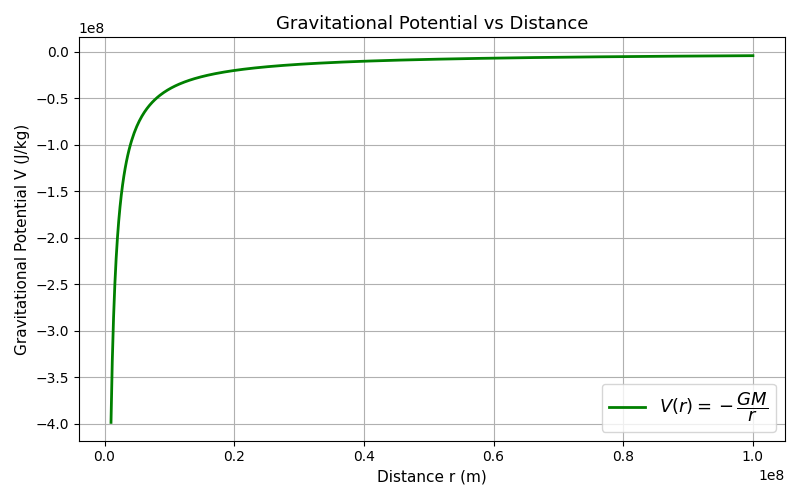
\includegraphics[width=0.7\textwidth]{Figure_5.png}
    \caption{Scalar potential $\phi$}
    \label{fig:phi}
\end{figure}
\begin{figure}
    \centering
    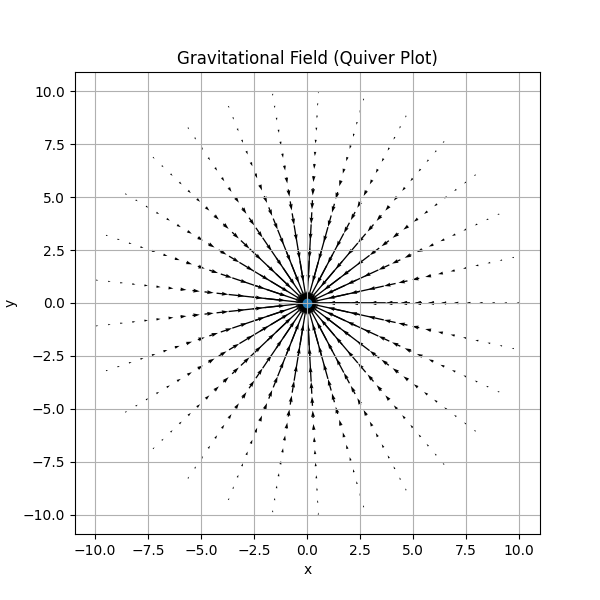
\includegraphics[width=0.7\textwidth]{Figure_1.png}
    \caption{Scalar field $\vec{g}$}
    \label{fig:g}
\end{figure}
\begin{figure}
    \centering
    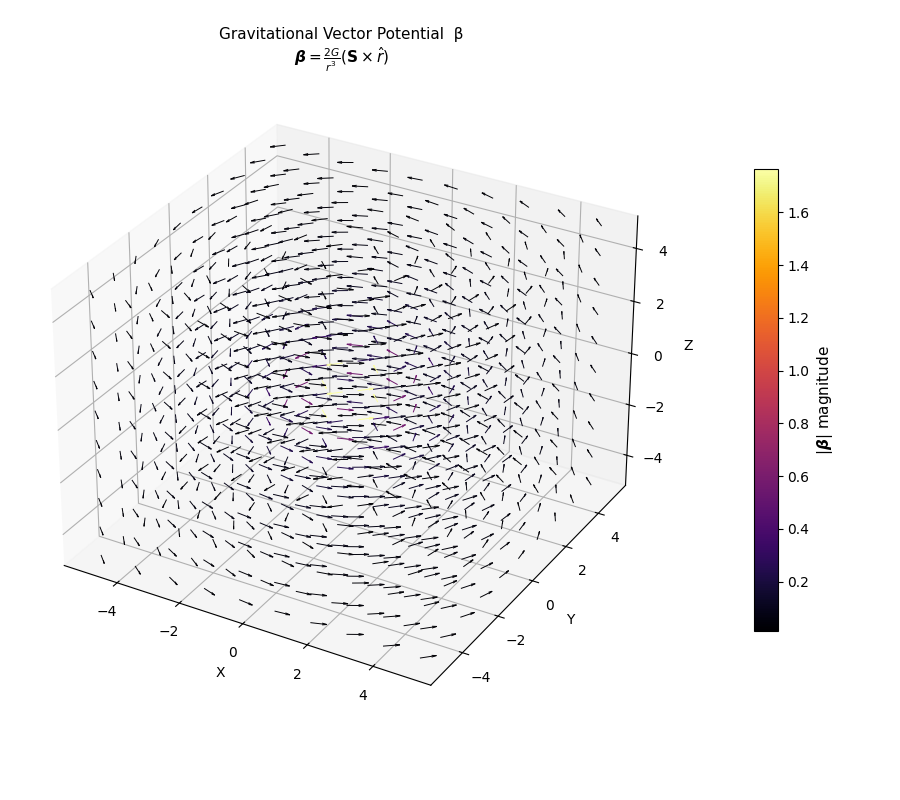
\includegraphics[width=0.7\textwidth]{Figure_2.png}
    \caption{vector potential $\vec{\beta}$}
    \label{fig:beta}
\end{figure}
\begin{figure}
    \centering
    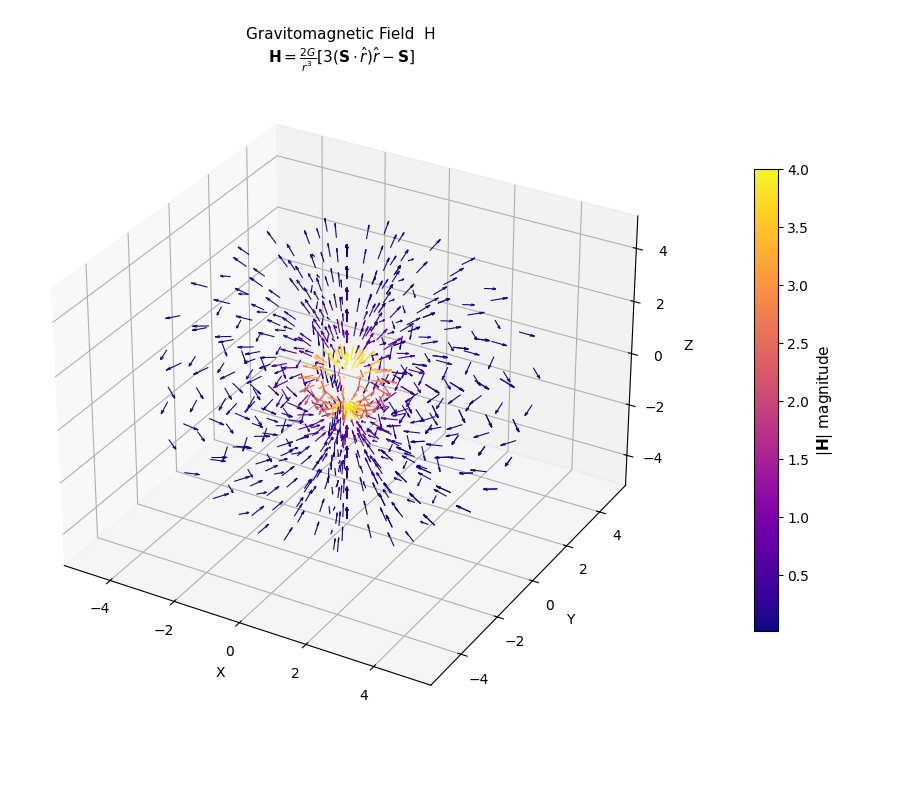
\includegraphics[width=0.7\textwidth]{Figure_3.png}
    \caption{vector field $\vec{H}$}
    \label{fig:H}
\end{figure}
% ============================================================
\newpage
\section{Results}
The precession produced by the gravitomagnetic field is extremely small, making it difficult to detect without highly sensitive instruments. As a result, the resulting shift in the orbital angle of a satellite occurs very slowly over time. The \ref{fig:orb} figure illustrates the evolution of the orbital precession, showing how the angular position gradually changes over an extended time scale. This demonstrates that the frame-dragging effect predicted by the Lense–Thirring mechanism produces only a minute deviation in the orbit. The \ref{fig:F} figure presents the effective force field acting on a satellite in an inclined orbit. The field structure closely resembles the conventional gravitational field, indicating that the dominant contribution arises from the Newtonian component of gravity. Because the gravitomagnetic contribution is extremely weak, only a very small perturbation to the overall field can be observed.

\begin{figure}
    \centering
    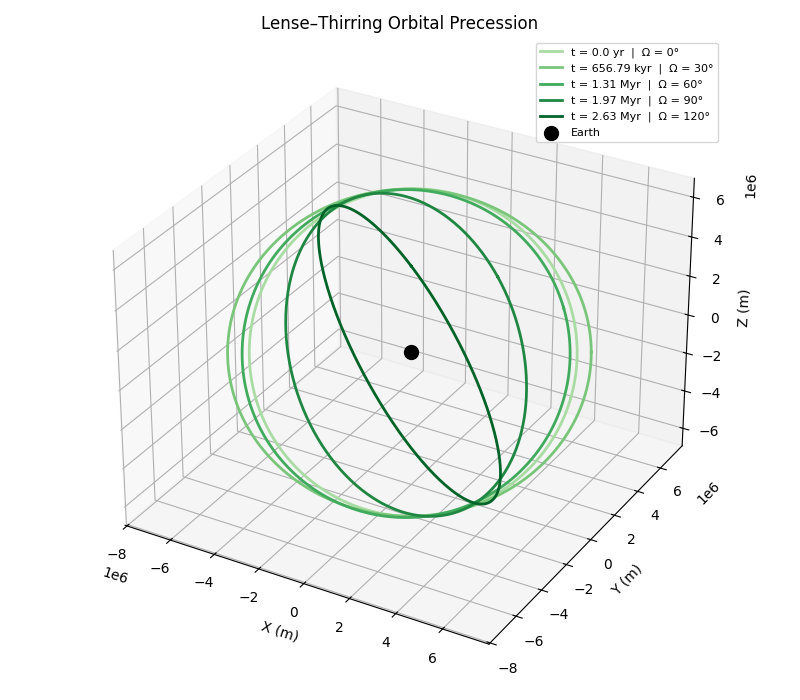
\includegraphics[width=0.7\textwidth]{Figure_4.png}
    \caption{Lense-Thirring Precession}
    \label{fig:orb}
\end{figure}
\begin{figure}
    \centering
    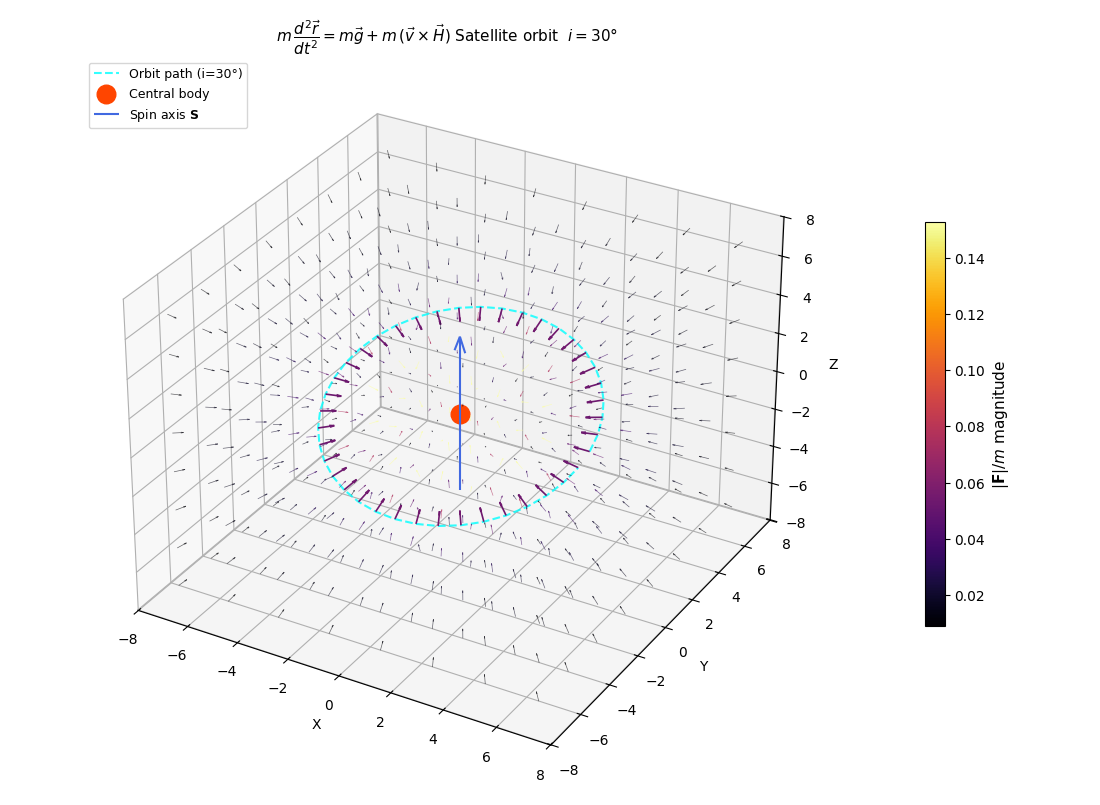
\includegraphics[width=0.7\textwidth]{Figure_6.png}
    \caption{Effective Field}
    \label{fig:F}
\end{figure}
% ============================================================
\section{Discussion}
\label{sec:discussion}
% ============================================================
An important experimental verification of the Lense–Thirring frame-dragging effect predicted by general relativity has been performed using the LAGEOS satellites orbiting Earth. These satellites allow extremely precise measurements of orbital motion through laser ranging techniques. According to the theoretical prediction of General Relativity, the rotation of Earth should produce a small precession of the orbital plane due to the Lense–Thirring effect. The predicted frame-dragging precession for the LAGEOS satellites is approximately **31 milliarcseconds per year**, while experimental measurements have reported a value of roughly **31 ± 2 milliarcseconds per year**. The small discrepancies between theoretical and measured values arise partly from simplifying assumptions in the model, such as treating Earth as a perfectly spherical mass distribution, whereas in reality the planet exhibits deviations from spherical symmetry. Despite these small uncertainties, the measurements show strong agreement with the theoretical prediction and provide important observational support for general relativity. This weak-field approximation analysis also illustrates how complex gravitational equations can be simplified using techniques such as linearization and gauge transformations, revealing a mathematical structure analogous to that of electromagnetism in the weak-field limit.

\newpage
% ============================================================








\newpage
% ── Bibliography ─────────────────────────────────────────────
\begin{thebibliography}{99}

\bibitem{einstein1916}
A. Einstein, ``Die Grundlage der allgemeinen Relativit\"{a}tstheorie,''
\textit{Annalen der Physik}, vol.~354, no.~7, pp.~769--822, 1916.

\bibitem{Lense1918}
J. Lense and H. Thirring, ``\"{U}ber den Einfluss der Eigenrotation der Zentralk\"{o}rper auf die Bewegung der Planeten und Monde nach der Einsteinschen Gravitationstheorie,''
\textit{Physikalische Zeitschrift}, vol.~19, pp.~156--163, 1918.

\bibitem{mashhoon1984}
B. Mashhoon, F.~W. Hehl, and D.~S. Theiss, ``On the gravitational effects of rotating masses: The Thirring-Lense papers,''
\textit{General Relativity and Gravitation}, vol.~16, no.~8, pp.~711--750, 1984.

\bibitem{mtw1973}
C.~W. Misner, K.~S. Thorne, and J.~A. Wheeler,
\textit{Gravitation}.
San Francisco: W.~H. Freeman, 1973.

\bibitem{carroll2004}
S. Carroll,
\textit{Spacetime and Geometry: An Introduction to General Relativity}.
San Francisco: Addison-Wesley, 2004.

\bibitem{wald1984}
R.~M. Wald,
\textit{General Relativity}.
Chicago: University of Chicago Press, 1984.

\bibitem{pfister2007}
H. Pfister, ``On the history of the so-called Lense-Thirring effect,''
\textit{General Relativity and Gravitation}, vol.~39, no.~11, pp.~1735--1748, 2007.

\bibitem{ciufolini1995}
I. Ciufolini and J.~A. Wheeler,
\textit{Gravitation and Inertia}.
Princeton: Princeton University Press, 1995.

\bibitem{ciufolini2004}
I. Ciufolini and E.~C. Pavlis, ``A confirmation of the general relativistic prediction of the Lense-Thirring effect,''
\textit{Nature}, vol.~431, pp.~958--960, 2004.

\bibitem{ciufolini1998}
I. Ciufolini, E.~C. Pavlis, F. Chieppa, E. Fernandes-Vieira, and J. P\'{e}rez-Mercader,
``Test of general relativity and measurement of the Lense-Thirring effect with two Earth satellites,''
\textit{Science}, vol.~279, no.~5359, pp.~2100--2103, 1998.

\bibitem{iorio2011}
L. Iorio, H.~I.~M. Lichtenegger, M.~L. Ruggiero, and C. Corda,
``Phenomenology of the Lense-Thirring effect in the Solar System,''
\textit{Astrophysics and Space Science}, vol.~331, no.~2, pp.~351--395, 2011.

\bibitem{mashhoon2007}
B. Mashhoon, ``Gravitoelectromagnetism: A Brief Review,''
in \textit{The Measurement of Gravitomagnetism: A Challenging Enterprise},
L. Iorio, Ed. New York: Nova Science, 2007, pp.~29--39.

\bibitem{hartle2003}
J.~B. Hartle,
\textit{Gravity: An Introduction to Einstein's General Relativity}.
San Francisco: Addison-Wesley, 2003.

\end{thebibliography}
\newpage
% ── Appendix ─────────────────────────────────────────────────
\appendix

\section*{Appendix: Python Code for Field Visualizations}

\subsection*{A.1 Gravitational Potential}

\begin{lstlisting}[language=Python]
import numpy as np
import matplotlib.pyplot as plt

G = 6.67430e-11
M = 5.972e24

r = np.linspace(1e6, 1e8, 500)

V = -G * M / r

fig, ax = plt.subplots(figsize=(8, 5))

ax.plot(r, V, label=r'$V(r) = -\dfrac{GM}{r}$', linewidth=2, color='green')

ax.set_xlabel("Distance r (m)", fontsize=11)
ax.set_ylabel("Gravitational Potential V (J/kg)", fontsize=11)
ax.set_title("Gravitational Potential vs Distance", fontsize=13)
ax.legend(fontsize=13)
ax.grid(True)

plt.tight_layout()
plt.show()
\end{lstlisting}

\subsection*{A.2 Gravitational Field}

\begin{lstlisting}[language=Python]
import numpy as np
import matplotlib.pyplot as plt

# Constants
G = 6.67430e-11
M = 5.972e24

# Polar grid
r = np.linspace(2, 10, 15)
theta = np.linspace(0, 2*np.pi, 30)

R, T = np.meshgrid(r, theta)

# Convert to Cartesian positions
X = R * np.cos(T)
Y = R * np.sin(T)

# Gravitational field magnitude
g = -G*M / R**2

# Field components
gx = g * np.cos(T)
gy = g * np.sin(T)

# Rescale for visualization
gx /= np.max(np.abs(gx))
gy /= np.max(np.abs(gy))

# Plot
plt.figure(figsize=(6,6))
plt.quiver(X, Y, gx, gy)
plt.scatter(0, 0)
plt.xlabel("x")
plt.ylabel("y")
plt.title("Gravitational Field (Quiver Plot)")
plt.axis("equal")
plt.grid('on')
plt.show()
\end{lstlisting}

\subsection*{A.3 Gravitomagnetic Vector Potential $\boldsymbol{\beta}$}

\begin{lstlisting}[language=Python]
import numpy as np
import matplotlib.pyplot as plt
from matplotlib.colors import Normalize
from matplotlib.cm import ScalarMappable

G = 1.0
S = np.array([0, 0, 1])

x = np.linspace(-5, 5, 10)
y = np.linspace(-5, 5, 10)
z = np.linspace(-5, 5, 10)

X, Y, Z = np.meshgrid(x, y, z)

R = np.sqrt(X**2 + Y**2 + Z**2)
R[R == 0] = 1e-6

Bx = S[1]*Z - S[2]*Y
By = S[2]*X - S[0]*Z
Bz = S[0]*Y - S[1]*X

Bx = (2*G / R**3) * Bx
By = (2*G / R**3) * By
Bz = (2*G / R**3) * Bz

magnitude = np.sqrt(Bx**2 + By**2 + Bz**2).ravel()

x_f  = X.ravel();  y_f  = Y.ravel();  z_f  = Z.ravel()
bx_f = Bx.ravel(); by_f = By.ravel(); bz_f = Bz.ravel()

nm = np.sqrt(bx_f**2 + by_f**2 + bz_f**2)
nm[nm == 0] = 1
bx_n = bx_f / nm
by_n = by_f / nm
bz_n = bz_f / nm

cmap  = plt.cm.inferno
vmin, vmax = magnitude.min(), magnitude.max()
cnorm  = Normalize(vmin=vmin, vmax=vmax)
colors = cmap(cnorm(magnitude))

fig = plt.figure(figsize=(9, 8))
ax  = fig.add_subplot(111, projection='3d')

for xi, yi, zi, ux, uy, uz, col in zip(x_f, y_f, z_f,
                                        bx_n, by_n, bz_n, colors):
    ax.quiver(xi, yi, zi, ux, uy, uz,
              length=0.45, normalize=False,
              color=col, linewidth=0.7, arrow_length_ratio=0.3)

sm = ScalarMappable(cmap=cmap, norm=cnorm)
sm.set_array([])
cbar = fig.colorbar(sm, ax=ax, shrink=0.6, pad=0.1)
cbar.set_label(r'$|\boldsymbol{\beta}|$ magnitude', fontsize=11)

ax.set_xlabel('X')
ax.set_ylabel('Y')
ax.set_zlabel('Z')
ax.set_title(r'Gravitational Vector Potential $\boldsymbol{\beta}$', fontsize=11)

plt.tight_layout()
plt.show()
\end{lstlisting}

\subsection*{A.4 Gravitomagnetic Field $\mathbf{H}$}

\begin{lstlisting}[language=Python]
import numpy as np
import matplotlib.pyplot as plt
from matplotlib.colors import Normalize
from matplotlib.cm import ScalarMappable

G = 1.0
S = np.array([0.0, 0.0, 1.0])

r     = np.linspace(1, 5, 6)
theta = np.linspace(0, np.pi, 12)
phi   = np.linspace(0, 2*np.pi, 12)

R, TH, PH = np.meshgrid(r, theta, phi)

X = R * np.sin(TH) * np.cos(PH)
Y = R * np.sin(TH) * np.sin(PH)
Z = R * np.cos(TH)

rx = X / R
ry = Y / R
rz = Z / R

Sdotr = S[0]*rx + S[1]*ry + S[2]*rz

Hx = (2*G / R**3) * (3*Sdotr*rx - S[0])
Hy = (2*G / R**3) * (3*Sdotr*ry - S[1])
Hz = (2*G / R**3) * (3*Sdotr*rz - S[2])

magnitude = np.sqrt(Hx**2 + Hy**2 + Hz**2)

x_f  = X.ravel();  y_f  = Y.ravel();  z_f  = Z.ravel()
hx_f = Hx.ravel(); hy_f = Hy.ravel(); hz_f = Hz.ravel()
mag  = magnitude.ravel()

norm_mag = np.sqrt(hx_f**2 + hy_f**2 + hz_f**2)
norm_mag[norm_mag == 0] = 1
hx_n = hx_f / norm_mag
hy_n = hy_f / norm_mag
hz_n = hz_f / norm_mag

cmap = plt.cm.plasma
vmin, vmax = mag.min(), mag.max()
cnorm = Normalize(vmin=vmin, vmax=vmax)
colors = cmap(cnorm(mag))

fig = plt.figure(figsize=(9, 8))
ax  = fig.add_subplot(111, projection='3d')

for xi, yi, zi, ux, uy, uz, col in zip(x_f, y_f, z_f,
                                        hx_n, hy_n, hz_n, colors):
    ax.quiver(xi, yi, zi, ux, uy, uz,
              length=0.45, normalize=False,
              color=col, linewidth=0.8, arrow_length_ratio=0.3)

sm = ScalarMappable(cmap=cmap, norm=cnorm)
sm.set_array([])
cbar = fig.colorbar(sm, ax=ax, shrink=0.6, pad=0.1)
cbar.set_label(r'$|\mathbf{H}|$ magnitude', fontsize=11)

ax.set_xlabel('X')
ax.set_ylabel('Y')
ax.set_zlabel('Z')
ax.set_title(r'Gravitomagnetic Field $\mathbf{H}$', fontsize=11)

plt.tight_layout()
plt.show()
\end{lstlisting}

\subsection*{A.5 Lense--Thirring Orbital Precession}

\begin{lstlisting}[language=Python]
import numpy as np
import matplotlib.pyplot as plt

G = 6.67430e-11
c = 299792458

M = 5.972e24
R = 6.371e6
omega = 7.292115e-5
I = 0.33 * M * R**2
S = I * omega

a = 7e6
e = 0.01
i = np.radians(60)

Omega_LT = 2 * G * S / (c**2 * a**3 * (1 - e**2)**1.5)

theta = np.linspace(0, 2 * np.pi, 400)
r = a * (1 - e**2) / (1 + e * np.cos(theta))

fig = plt.figure(figsize=(8, 7))
ax = fig.add_subplot(111, projection='3d')

delta_deg = 30
delta_rad = np.radians(delta_deg)
seconds_per_step = delta_rad / Omega_LT
years_per_step = seconds_per_step / (3600 * 24 * 365.25)

time_steps = [0, 1, 2, 3, 4]
colors = plt.cm.Greens(np.linspace(0.35, 0.9, len(time_steps)))

for idx, t in enumerate(time_steps):
    Omega = np.radians(delta_deg * t)

    x = r * np.cos(theta)
    y = r * np.sin(theta)

    y_i = y * np.cos(i)
    z_i = y * np.sin(i)

    xp = x * np.cos(Omega) - y_i * np.sin(Omega)
    yp = x * np.sin(Omega) + y_i * np.cos(Omega)
    zp = z_i

    elapsed_years = t * years_per_step
    if elapsed_years >= 1e6:
        time_str = f"{elapsed_years/1e6:.2f} Myr"
    elif elapsed_years >= 1e3:
        time_str = f"{elapsed_years/1e3:.2f} kyr"
    else:
        time_str = f"{elapsed_years:.1f} yr"

    ax.plot(xp, yp, zp, linewidth=2, color=colors[idx],
            label=f"t = {time_str}  |  Omega = {delta_deg*t} deg")

ax.scatter(0, 0, 0, s=100, color='black', zorder=10, label='Earth')

ax.set_xlabel("X (m)")
ax.set_ylabel("Y (m)")
ax.set_zlabel("Z (m)")
ax.set_title("Lense-Thirring Orbital Precession")
ax.legend(fontsize=8)

plt.tight_layout()
plt.show()

\subsection*{A.6 Effective Force Field on Inclined Satellite Orbit}

\begin{lstlisting}[language=Python]
import numpy as np
import matplotlib.pyplot as plt
from matplotlib.colors import Normalize
from matplotlib.cm import ScalarMappable

# Constants (normalized)
G = 1.0
M = 1.0
S = np.array([0.0, 0.0, 1.0])   # spin along z
a = 5.0                           # orbital radius
i = np.radians(30)                # inclination from equatorial plane

# Orbit: parametric position & velocity
N = 40
phi = np.linspace(0, 2*np.pi, N, endpoint=False)

X_orb = a * np.cos(phi)
Y_orb = a * np.sin(phi) * np.cos(i)
Z_orb = a * np.sin(phi) * np.sin(i)

v_mag = np.sqrt(G * M / a)
Vx_orb = -v_mag * np.sin(phi)
Vy_orb =  v_mag * np.cos(phi) * np.cos(i)
Vz_orb =  v_mag * np.cos(phi) * np.sin(i)

# 3D grid of field points
gx_ = np.linspace(-7, 7, 8)
gy_ = np.linspace(-7, 7, 8)
gz_ = np.linspace(-7, 7, 8)
Xg, Yg, Zg = np.meshgrid(gx_, gy_, gz_)

Rg = np.sqrt(Xg**2 + Yg**2 + Zg**2)
Rg[Rg < 1.0] = 1e-6

rxg = Xg/Rg; ryg = Yg/Rg; rzg = Zg/Rg

v_grid = np.sqrt(G * M / Rg)
phi_g = np.arctan2(Yg, Xg)
Vxg = -v_grid * np.sin(phi_g)
Vyg =  v_grid * np.cos(phi_g)
Vzg =  np.zeros_like(Vxg)

# g field on grid
gm_g = G * M / Rg**2
gxg = -gm_g * rxg;  gyg = -gm_g * ryg;  gzg = -gm_g * rzg

# H field on grid
Sdotrg = S[0]*rxg + S[1]*ryg + S[2]*rzg
Hp_g = 4*G / Rg**3
Hxg = Hp_g*(3*Sdotrg*rxg - S[0])
Hyg = Hp_g*(3*Sdotrg*ryg - S[1])
Hzg = Hp_g*(3*Sdotrg*rzg - S[2])

# v x H on grid
vxHxg = Vyg*Hzg - Vzg*Hyg
vxHyg = Vzg*Hxg - Vxg*Hzg
vxHzg = Vxg*Hyg - Vyg*Hxg

Fxg = gxg + vxHxg;  Fyg = gyg + vxHyg;  Fzg = gzg + vxHzg
Fmg = np.sqrt(Fxg**2 + Fyg**2 + Fzg**2)
Fmg[Fmg == 0] = 1e-9

Fxg_n = Fxg/Fmg;  Fyg_n = Fyg/Fmg;  Fzg_n = Fzg/Fmg

# Orbital force
R_orb = a
rx_o = X_orb/R_orb; ry_o = Y_orb/R_orb; rz_o = Z_orb/R_orb
gm_o = G*M/R_orb**2
gxo = -gm_o*rx_o; gyo = -gm_o*ry_o; gzo = -gm_o*rz_o
Sdotro = S[0]*rx_o + S[1]*ry_o + S[2]*rz_o
Hp_o = 4*G/R_orb**3
Hxo = Hp_o*(3*Sdotro*rx_o - S[0])
Hyo = Hp_o*(3*Sdotro*ry_o - S[1])
Hzo = Hp_o*(3*Sdotro*rz_o - S[2])
vxHxo = Vy_orb*Hzo - Vz_orb*Hyo
vxHyo = Vz_orb*Hxo - Vx_orb*Hzo
vxHzo = Vx_orb*Hyo - Vy_orb*Hxo
Fxo = gxo+vxHxo; Fyo = gyo+vxHyo; Fzo = gzo+vxHzo
Fmo = np.sqrt(Fxo**2+Fyo**2+Fzo**2)
Fxo_n = Fxo/Fmo; Fyo_n = Fyo/Fmo; Fzo_n = Fzo/Fmo

# Combined magnitude range for single colourbar
all_mag = np.concatenate([Fmg.ravel(), Fmo])

# Plot
cmap  = plt.cm.inferno
cnorm = Normalize(vmin=np.percentile(all_mag, 5),
                  vmax=np.percentile(all_mag, 95))

fig = plt.figure(figsize=(11, 9))
ax  = fig.add_subplot(111, projection='3d')

# Grid field arrows
xf = Xg.ravel(); yf = Yg.ravel(); zf = Zg.ravel()
fxf = Fxg_n.ravel(); fyf = Fyg_n.ravel(); fzf = Fzg_n.ravel()
mf  = Fmg.ravel()
cols_grid = cmap(cnorm(mf))

for xi, yi, zi, ux, uy, uz, col in zip(xf, yf, zf, fxf, fyf, fzf, cols_grid):
    ax.quiver(xi, yi, zi, ux, uy, uz,
              length=0.38, normalize=False,
              color=col, linewidth=0.5, arrow_length_ratio=0.25, alpha=0.6)

# Orbit path
ax.plot(X_orb, Y_orb, Z_orb, color='cyan', linewidth=1.5,
        linestyle='--', alpha=0.8, label='Orbit path (i=30 deg)')

# Orbital force arrows
cols_orb = cmap(cnorm(Fmo))
for xi, yi, zi, ux, uy, uz, col in zip(X_orb, Y_orb, Z_orb,
                                        Fxo_n, Fyo_n, Fzo_n, cols_orb):
    ax.quiver(xi, yi, zi, ux, uy, uz,
              length=0.6, normalize=False,
              color=col, linewidth=1.2, arrow_length_ratio=0.3)

# Central body and spin axis
ax.scatter(0, 0, 0, s=180, color='orangered', zorder=10, label='Central body')
ax.quiver(0, 0, -4, 0, 0, 8, color='royalblue', linewidth=1.5,
          arrow_length_ratio=0.1, label='Spin axis S')

# Colourbar
sm = ScalarMappable(cmap=cmap, norm=cnorm)
sm.set_array([])
cbar = fig.colorbar(sm, ax=ax, shrink=0.55, pad=0.1)
cbar.set_label(r'$|\mathbf{F}|/m$ magnitude', fontsize=11)

ax.set_xlabel('X');  ax.set_ylabel('Y');  ax.set_zlabel('Z')
ax.set_title(r'Effective Force Field: $m\,\frac{d^2\vec{r}}{dt^2}'
             r'= m\vec{g} + m\,(\vec{v}\times\vec{H})$', fontsize=11)
ax.legend(fontsize=9, loc='upper left')

plt.tight_layout()
plt.show()
\end{lstlisting}





% ============================================================
\end{document}
% ============================================================
